% Created 2019-05-27 Mon 11:49
\documentclass[9pt, b5paper]{article}
\usepackage[UTF8]{ctex}
\usepackage{fontspec}
\usepackage{graphicx}
\usepackage{xcolor}
\usepackage{multirow}
\usepackage{multicol}
\usepackage{float}
\usepackage{textcomp}
\usepackage{geometry}
\geometry{left=1.2cm,right=1.2cm,top=1.5cm,bottom=1.2cm}
\usepackage{algorithm}
\usepackage{algorithmic}
\usepackage{latexsym}
\usepackage{natbib}
\usepackage{listings}
\usepackage{minted}
\usepackage[xetex,colorlinks=true,CJKbookmarks=true,linkcolor=blue,urlcolor=blue,menucolor=blue]{hyperref}
\author{deepwaterooo}
\date{\today}
\title{Android Interview Preparation -- Coding}
\hypersetup{
  pdfkeywords={},
  pdfsubject={},
  pdfcreator={Emacs 26.1 (Org mode 8.2.7c)}}
\begin{document}

\maketitle
\tableofcontents


\section{全面了解Activity}
\label{sec-1}
\subsection{Activity是什么?}
\label{sec-1-1}
\begin{itemize}
\item 我们都知道android中有四大组件(Activity 活动,Service 服务,Content Provider 内容提供者,BroadcastReceiver 广播接收器),Activity是我们用的最多也是最基本的组件,因为应用的所有操作都与用户相关,Activity 提供窗口来和用户进行交互。
\end{itemize}
官方文档这么说:
\begin{itemize}
\item An activity is a single, focused thing that the user can do. Almost all activities interact with the user, so the Activity class takes care of creating a window for you in which you can place your UI with setContentView(View).
\item 大概的意思(原谅我):activity是独立平等的,用来处理用户操作。几乎所有的activity都是用来和用户交互的,所以activity类会创建了一个窗口,开发者可以通过setContentView(View)的接口把UI放到给窗口上。
\item Android中的activity全都归属于task管理 。task 是多个 activity 的集合,这些 activity 按照启动顺序排队存入一个栈(即“back stack”)。android默认会为每个App维持一个task来存放该app的所有activity,task的默认name为该app的packagename。
\item 当然我们也可以在AndroidMainfest.xml中申明activity的taskAffinity属性来自定义task,但不建议使用,如果其他app也申明相同的task,它就有可能启动到你的activity,带来各种安全问题(比如拿到你的Intent)。
\end{itemize}
\subsection{Activity的内部调用过程}
\label{sec-1-2}
\begin{itemize}
\item 上面已经说了,系统通过堆栈来管理activity,当一个新的activity开始时,它被放置在堆栈的顶部和成为运行活动,以前的activity始终保持低于它在堆栈,而不会再次到达前台,直到新的活动退出。
\item 还是上这张官网的activity\_lifecycle图:
\item ![这里写图片描述](\url{http://img.blog.csdn.net/20160425171711054}) 
\item 首先打开一个新的activity实例的时候,系统会依次调用
\begin{itemize}
\item -> onCreate()  -> onStart() -> onResume() 然后开始running
\end{itemize}
\item running的时候被覆盖了(从它打开了新的activity或是被锁屏,但是它**依然在前台**运行, lost focus but is still visible),系统调用onPause();
\begin{itemize}
\item 该方法执行activity暂停,通常用于提交未保存的更改到持久化数据,停止动画和其他的东西。但这个activity还是完全活着(它保持所有的状态和成员信息,并保持连接到**窗口管理器**)
\end{itemize}
\item 接下来它有三条出路
\begin{itemize}
\item ①用户返回到该activity就调用onResume()方法重新running
\item ②用户回到桌面或是打开其他activity,就会调用onStop()进入停止状态(保留所有的状态和成员信息,**对用户不可见**)
\item ③系统内存不足,拥有更高限权的应用需要内存,那么该activity的进程就可能会被系统回收。(回收onRause()和onStop()状态的activity进程)要想重新打开就必须重新创建一遍。
\end{itemize}
\end{itemize}
如果用户返回到onStop()状态的activity(又显示在前台了),系统会调用
> onRestart() ->  onStart() -> onResume() 然后重新running
在activity结束(调用finish ())或是被系统杀死之前会调用onDestroy()方法释放所有占用的资源。

\begin{itemize}
\item activity生命周期中三个嵌套的循环
\begin{itemize}
\item activity的完整生存期会在 onCreate() 调用和 onDestroy() 调用之间发生。 
\item activity的可见生存期会在 onStart() 调用和 onStop() 调用之间发生。系统会在activity的整个生存期内多次调用 onStart() 和onStop(), 因为activity可能会在显示和隐藏之间不断地来回切换。 
\item activity的前后台切换会在 onResume() 调用和 onPause() 之间发生。
\end{itemize}
\item 因为这个状态可能会经常发生转换,为了避免切换迟缓引起的用户等待,这两个方法中的代码应该相当地轻量化。
\end{itemize}
\subsubsection{activity被回收的状态和信息保存和恢复过程}
\label{sec-1-2-1}
\begin{minted}[linenos=true]{java}
public class MainActivity extends Activity {
    @Override
    protected void onCreate(Bundle savedInstanceState) {
        if (savedInstanceState != null){ // 判断是否有以前的保存状态信息
            savedInstanceState.get("Key"); 
        }
        super.onCreate(savedInstanceState);
        setContentView(R.layout.activity_main);
    }
    @Override
    protected void onSaveInstanceState(Bundle outState) {
        // TODO Auto-generated method stub
        // 可能被回收内存前保存状态和信息,
        Bundle data = new Bundle(); 
        data.putString("key", "last words before be kill");
        outState.putAll(data);
        super.onSaveInstanceState(outState);
    }
    @Override
    protected void onRestoreInstanceState(Bundle savedInstanceState) {
        // TODO Auto-generated method stub
        if (savedInstanceState != null){ // 判断是否有以前的保存状态信息
            savedInstanceState.get("Key"); 
        }
        super.onRestoreInstanceState(savedInstanceState);
    }
}
\end{minted}
\begin{enumerate}
\item onSaveInstanceState()方法
\label{sec-1-2-1-1}
\begin{itemize}
\item 在activity可能被回收之前调用,用来保存自己的状态和信息,以便回收后重建时恢复数据(在onCreate()或onRestoreInstanceState()中恢复)。旋转屏幕重建activity会调用该方法,但其他情况在onRause()和onStop()状态的activity不一定会调用 ,下面是该方法的文档说明。
\item One example of when onPause() and onStop() is called and not this method is when a user navigates back from activity B to activity A: there is no need to call onSaveInstanceState() on B because that particular instance will never be restored, so the system avoids calling it. An example when onPause() is called and not onSaveInstanceState() is when activity B is launched in front of activity A: the system may avoid calling onSaveInstanceState() on activity A if it isn't killed during the lifetime of B since the state of the user interface of A will stay intact.
\item 也就是说,系统灵活的来决定调不调用该方法, \textbf{但是如果要调用就一定发生在onStop()方法之前,但并不保证发生在onPause()的前面还是后面。}
\end{itemize}
\item onRestoreInstanceState()方法
\label{sec-1-2-1-2}
\begin{itemize}
\item 这个方法在onStart() 和 onPostCreate()之间调用,在onCreate()中也可以状态恢复,但有时候需要所有布局初始化完成后再恢复状态。
\item onPostCreate():一般不实现这个方法,当程序的代码开始运行时,它调用系统做最后的初始化工作。
\end{itemize}
\end{enumerate}
\subsection{启动模式}
\label{sec-1-3}
\subsubsection{启动模式什么?}
\label{sec-1-3-1}
\begin{itemize}
\item 简单的说就是定义activity 实例与task 的关联方式。
\end{itemize}
\subsubsection{为什么要定义启动模式?}
\label{sec-1-3-2}
\begin{itemize}
\item 为了实现一些默认启动(standard)模式之外的需求:
\begin{itemize}
\item 让某个 activity 启动一个新的 task (而不是被放入当前 task )
\item 让 activity 启动时只是调出已有的某个实例(而不是在 back stack 顶创建一个新的实例) 
\item 或者,你想在用户离开 task 时只保留根 activity,而 back stack 中的其它 activity 都要清空
\end{itemize}
\end{itemize}
\subsubsection{怎样定义启动模式?}
\label{sec-1-3-3}
\begin{itemize}
\item 定义启动模式的方法有两种:
\end{itemize}
\begin{enumerate}
\item 使用 manifest 文件
\label{sec-1-3-3-1}
\begin{itemize}
\item 在 manifest 文件中activity声明时,利用 activity 元素的 launchMode 属性来设定 activity 与 task 的关系。
\begin{minted}[linenos=true]{xml}
<activity
    android:launchMode="standard"
</activity>
\end{minted}
\item 注意: 你用 launchMode 属性为 activity 设置的模式可以被启动 activity 的 intent 标志所覆盖。
\end{itemize}
\begin{enumerate}
\item 有哪些启动模式?
\label{sec-1-3-3-1-1}
\begin{itemize}
\item "standard" (默认模式) 
\begin{itemize}
\item 当通过这种模式来启动Activity时,Android总会为目标Activity创建一个新的实例,并将该Activity添加到当前Task栈中。这种方式不会启动新的Task,只是将新的 Activity添加到原有的Task中。 
\end{itemize}
\item "singleTop" 
\begin{itemize}
\item 该模式和standard模式基本一致,但有一点不同:当将要被启动的Activity已经位于Task栈顶时,系统不会重新创建目标Activity实例,而是直接复用Task栈顶的Activity。
\end{itemize}
\item "singleTask"
\begin{itemize}
\item Activity在同一个Task内只有一个实例。
\item 如果将要启动的Activity不存在,那么系统将会创建该实例,并将其加入Task栈顶; 
\item 如果将要启动的Activity已存在,且存在栈顶,直接复用Task栈顶的Activity。 
\item 如果Activity存在但是没有位于栈顶,那么此时系统会把位于该Activity上面的所有其他Activity全部移出Task,从而使得该目标Activity位于栈顶。
\end{itemize}
\item "singleInstance" 
\begin{itemize}
\item 无论从哪个Task中启动目标Activity,只会创建一个目标Activity实例且会用一个全新的Task栈来装载该Activity实例(全局单例).
\item 如果将要启动的Activity不存在,那么系统将会先创建一个全新的Task,再创建目标Activity实例并将该Activity实例放入此全新的Task中。
\item 如果将要启动的Activity已存在,那么无论它位于哪个应用程序,哪个Task中;系统都会把该Activity所在的Task转到前台,从而使该Activity显示出来。
\end{itemize}
\end{itemize}
\end{enumerate}
\item 使用 Intent 标志
\label{sec-1-3-3-2}
\begin{itemize}
\item 在要启动 activity 时,你可以在传给 startActivity() 的 intent 中包含相应标志,以修改 activity 与 task 的默认关系。
\end{itemize}
\begin{minted}[linenos=true]{java}
Intent i = new Intent(this,NewActivity.class);
i.setFlags(Intent.FLAG_ACTIVITY_NEW_TASK);
startActivity(i);
\end{minted}
\begin{enumerate}
\item 可以通过标志修改的默认模式有哪些?
\label{sec-1-3-3-2-1}
\begin{itemize}
\item FLAG\_ACTIVITY\_NEW\_TASK
\begin{itemize}
\item 与"singleTask"模式相同,在新的 task 中启动 activity。如果要启动的 activity 已经运行于某 task 中,则那个 task 将调入前台。
\end{itemize}
\item FLAG\_ACTIVITY\_SINGLE\_TOP
\begin{itemize}
\item 与 "singleTop"模式相同,如果要启动的 activity位于back stack 顶,系统不会重新创建目标Activity实例,而是直接复用Task栈顶的Activity。
\end{itemize}
\item FLAG\_ACTIVITY\_CLEAR\_TOP
\begin{itemize}
\item 此种模式在launchMode中没有对应的属性值。
\item 如果要启动的 activity 已经在当前 task 中运行,则不再启动一个新的实例,且所有在其上面的 activity 将被销毁。
\end{itemize}
\end{itemize}
\item 关于启动模式的一些建议
\label{sec-1-3-3-2-2}
\begin{itemize}
\item 一般不要改变 activity 和 task 默认的工作方式。 如果你确定有必要修改默认方式,请保持谨慎,并确保 activity 在启动和从其它 activity 返回时的可用性,多做测试和安全方面的工作。
\end{itemize}
\end{enumerate}
\end{enumerate}
\subsection{Intent Filter}
\label{sec-1-4}
\begin{itemize}
\item android的3个核心组件——Activity、services、广播接收器——是通过intent传递消息的。intent消息用于在运行时绑定不同的组件。
\item 在 Android 的 AndroidManifest.xml 配置文件中可以通过 intent-filter 节点为一个 Activity 指定其 Intent Filter,以便告诉系统该 Activity 可以响应什么类型的 Intent。
\end{itemize}
\subsubsection{intent-filter 的三大属性}
\label{sec-1-4-1}
\begin{enumerate}
\item Action
\label{sec-1-4-1-1}
\begin{itemize}
\item 一个 Intent Filter 可以包含多个 Action,Action 列表用于标示 Activity 所能接受的“动作”,它是一个用户自定义的字符串。
\begin{minted}[linenos=true]{xml}
<intent-filter > 
 <action android:name="android.intent.action.MAIN" /> 
 <action android:name="com.scu.amazing7Action" /> 
……
 </intent-filter>
\end{minted}
\end{itemize}
在代码中使用以下语句便可以启动该Intent 对象:
Intent i=new Intent(); 
i.setAction("com.scu.amazing7Action");
Action 列表中包含了“com.scu.amazing7Action”的 Activity 都将会匹配成功
\item URL
\label{sec-1-4-1-2}
在 intent-filter 节点中,通过 data节点匹配外部数据,也就是通过 URI 携带外部数据给目标组件。
<data android:mimeType="mimeType" 
    android:scheme="scheme" 
     android:host="host"
     android:port="port" 
     android:path="path"/>
注意:只有data的所有的属性都匹配成功时 URI 数据匹配才会成功
\item Category
\label{sec-1-4-1-3}
为组件定义一个 类别列表,当 Intent 中包含这个类别列表的所有项目时才会匹配成功。
<intent-filter . . . >
   <action android:name="code android.intent.action.MAIN" />
   <category android:name="code android.intent.category.LAUNCHER" />
</intent-filter>
\end{enumerate}
\subsubsection{Activity 种 Intent Filter 的匹配过程}
\label{sec-1-4-2}
①加载所有的Intent Filter列表
②去掉action匹配失败的Intent Filter
③去掉url匹配失败的Intent Filter
④去掉Category匹配失败的Intent Filter
⑤判断剩下的Intent Filter数目是否为0。如果为0查找失败返回异常;如果大于0,就按优先级排序,返回最高优先级的Intent Filter

\subsection{开发中Activity的一些问题}
\label{sec-1-5}
\begin{itemize}
\item 一般设置Activity为非公开的
\begin{minted}[linenos=true]{xml}
<activity  
android:exported="false" />
\end{minted}
\item 注意:非公开的Activity不能设置intent-filter,以免被其他activity唤醒(如果拥有相同的intent-filter)。
\begin{itemize}
\item 不要指定activity的taskAffinity属性
\item 不要设置activity的LaunchMode(保持默认)
\end{itemize}
\item 注意Activity的intent最好也不要设定为FLAG\_ACTIVITY\_NEW\_TASK
\begin{itemize}
\item 在匿名内部类中使用this时加上activity类名(类名.this, 不一定是当前activity)
\item 设置activity全屏
\begin{itemize}
\item 在其 onCreate()方法中加入:
\end{itemize}
\begin{minted}[linenos=true]{java}
// 设置全屏模式
 getWindow().setFlags(WindowManager.LayoutParams.FLAG_FULLSCREEN, WindowManager.LayoutParams.FLAG_FULLSCREEN); 
 // 去除标题栏
 requestWindowFeature(Window.FEATURE_NO_TITLE);
\end{minted}
\end{itemize}
\end{itemize}

\section{Fragment全解析}
\label{sec-2}
\subsection{概述}
\label{sec-2-1}
\begin{itemize}
\item Fragment是Activity中用户界面的一个行为或者是一部分。主要是支持在大屏幕上动态和更为灵活的去组合或是交换UI组件,通过将activity的布局分割成若干个fragment,可以在运行时编辑activity的呈现,并且那些变化会被保存在由activity管理的后台栈里面。
\item \textbf{Fragment必须总是被嵌入到一个activity之中} ,并且fragment的生命周期直接受其宿主activity的生命周期的影响。你可以认为fragment是activity的一个模块零件,它有自己的生命周期,接收它自己的输入事件,并且可以在activity运行时添加或者删除。
\item 应该将每一个fragment设计为模块化的和可复用化的activity组件。也就是说,你可以在多个activity中引用同一个fragment,因为fragment定义了它自己的布局,并且使用它本身生命周期回调的行为。
\end{itemize}
\subsection{Fragment的生命周期}
\label{sec-2-2}
\begin{itemize}
\item 先看fragment生命周期图:

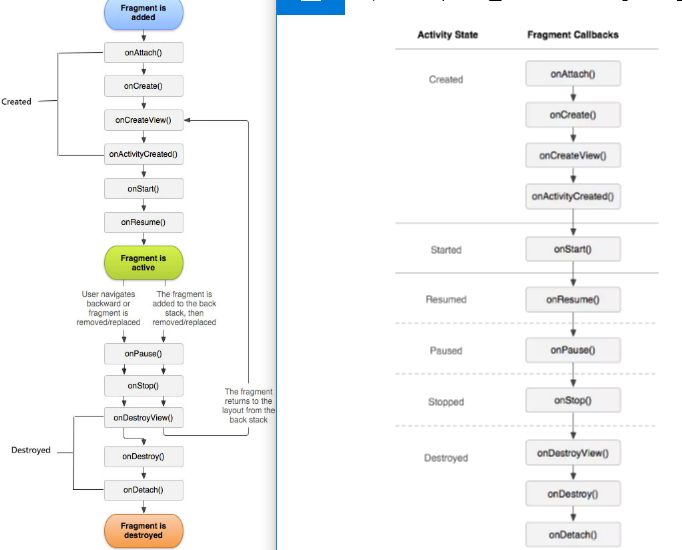
\includegraphics[width=.9\linewidth]{./pic/fragmentlifecycle2.png}
\item fragment所生存的activity生命周期直接影响着fragment的生命周期,由此针对activity的每一个生命周期回调都会引发一个fragment类似的回调。例如,当activity接收到onPause()时,这个activity之中的每个fragment都会接收到onPause()。
\end{itemize}
[这有Activity的详细说明](\url{http://blog.csdn.net/amazing7/article/details/51244219})
\begin{itemize}
\item Fragment有一些额外的生命周期回调方法(创建和销毁fragment界面).
\begin{itemize}
\item onAttach()
\begin{itemize}
\item 当fragment被绑定到activity时调用(Activity会被传入)。
\end{itemize}
\item onCreateView()
\begin{itemize}
\item 将本身的布局构建到activity中去(fragment作为activity界面的一部分)
\end{itemize}
\item onActivityCreated()
\begin{itemize}
\item 当activity的onCreate()函数返回时被调用。
\end{itemize}
\item onDestroyView()
\begin{itemize}
\item 当与fragment关联的视图体系正被移除时被调用。
\end{itemize}
\item onDetach()
\begin{itemize}
\item 当fragment正与activity解除关联时被调用。
\end{itemize}
\end{itemize}
\item 当activity接收到它的onCreate()回调时,activity之中的fragment接收到onActivityCreated()回调。
\begin{itemize}
\item 一旦activity处于resumed状态,则可以在activity中自由的添加或者移除fragment。因此,只
\end{itemize}
\end{itemize}
\textbf{有当activity处于resumed状态时} ,fragment的生命周期才可以独立变化。fragment会在 activity离开恢复状态时 再一次被activity推入它的生命周期中。
\begin{itemize}
\item \textbf{管理fragment生命周期} 与管理activity生命周期很相像。像activity一样,fragment也有三种状态:
\begin{itemize}
\item Resumed
\begin{itemize}
\item fragment在运行中的activity可见。
\end{itemize}
\item Paused
\begin{itemize}
\item 另一个activity处于前台且得到焦点,但是这个fragment所在的activity仍然可见(前台activity部分透明,或者没有覆盖全屏)。
\end{itemize}
\item Stopped
\begin{itemize}
\item fragment不可见。要么宿主activity已经停止,要么fragment已经从activity上移除,但已被添加到后台栈中。一个停止的fragment仍然活着(所有状态和成员信息仍然由系统保留着)。但是,它对用户来讲已经不再可见,并且如果activity被杀掉,它也将被杀掉。
\item 如果activity的进程被杀掉了,在activity被重新创建时,你需要恢复fragment状态。可以执行fragment的onSaveInstanceState()来保存状态(注意在fragment是在onCreate(),onCreateView(),或onActvityCreate()中进行恢复)。
\end{itemize}
\end{itemize}
\item 在生命周期方面,activity与fragment之间一个 \textbf{很重要的不同} ,就是在各自的后台栈中是如何存储的。
\begin{itemize}
\item 当activity停止时,默认情况下activity被安置在由系统管理的activity后台栈中; 
\item fragment仅当在一个事务被移除时,通过显式调用addToBackStack()请求保存的实例,该fragment才被置于由宿主activity管理的后台栈。 
\end{itemize}
\item \textbf{要创建一个fragment} ,必须创建一个fragment的子类。一般情况下,我们至少需要实现以下几个fragment生命周期方法:
\begin{itemize}
\item onCreate()
\begin{itemize}
\item 在创建fragment时系统会调用此方法。在实现代码中,你可以初始化想要在fragment中保持的那些必要组件,当fragment处于暂停或者停止状态之后可重新启用它们。
\end{itemize}
\item onCreateView()
\begin{itemize}
\item 在第一次为fragment绘制用户界面时系统会调用此方法。为fragment绘制用户界面,这个函数必须要返回所绘出的fragment的根View。如果fragment没有用户界面可以返回空。
\end{itemize}
\end{itemize}
\begin{minted}[linenos=true]{java}
@Override
public View onCreateView(LayoutInflater inflater, ViewGroup container,
                         Bundle savedInstanceState) { 
    // Inflate the layout for this fragment
    return inflater.inflate(R.layout.example_fragment, container, false);
}
\end{minted}
\begin{itemize}
\item inflate()函数需要以下三个参数:
\begin{itemize}
\item ①要inflate的布局的资源ID。 
\item ②被inflate的布局的父ViewGroup。
\item ③一个布尔值,表明在inflate期间被infalte的布局是否应该附上ViewGroup(第二个参数container)。(在这个例子中传入的是false,因为系统已经将被inflate的布局插入到容器中(container)——传入true会在最终的布局里创建一个多余的ViewGroup。) 
\end{itemize}
\item onPause()
\begin{itemize}
\item 系统回调用该函数作为用户离开fragment的第一个预兆(尽管这并不总意味着fragment被销毁)。在当前用户会话结束之前,通常要在这里提交任何应该持久化的变化(因为用户可能不再返回)。
\end{itemize}
\end{itemize}
\end{itemize}

\subsection{将fragment添加到activity之中}
\label{sec-2-3}
\begin{itemize}
\item 可以通过在activity布局文件中声明fragment,用fragment标签把fragment插入到activity的布局中,或者是用应用程序源码将它添加到一个存在的ViewGroup中。 
\item 但fragment并不是一个定要作为activity布局的一部分,fragment也可以为activity隐身工作。
\end{itemize}
\subsubsection{在activity的布局文件里声明fragment}
\label{sec-2-3-1}
\begin{itemize}
\item 可以像为view一样为fragment指定布局属性。例如:
\begin{minted}[linenos=true]{xml}
<?xml version="1.0" encoding="utf-8"?>
<LinearLayout xmlns:android="http://schemas.android.com/apk/res/android"
      android:orientation="horizontal"
      android:layout_width="match_parent"
      android:layout_height="match_parent"> 
<fragment android:name="com.example.test.FragmentOne"
      android:id="@+id/fo"
      android:layout_width="match_parent"
      android:layout_height="match_parent" />
</LinearLayout>
\end{minted}
\item fragment标签中的android:name 属性指定了布局中实例化的Fragment类。
\item 当系统创建activity布局时,它实例化了布局文件中指定的每一个fragment,并为它们调用onCreateView()函数,以获取每一个fragment的布局。系统直接在<fragment>元素的位置插入fragment返回的View。
\item 注意:每个fragment都需要一个唯一的标识,如果重启activity,系统可用来恢复fragment(并且可用来捕捉fragment的事务处理,例如移除)。
\item 为fragment提供ID有三种方法:
\begin{itemize}
\item 用android:id属性提供一个唯一的标识。 
\item 用android:tag属性提供一个唯一的字符串。 
\item 如果上述两个属性都没有,系统会使用其容器视图(view)的ID。 
\end{itemize}
\end{itemize}
\subsubsection{通过编码将fragment添加到已存在的ViewGroup中}
\label{sec-2-3-2}
\begin{itemize}
\item 在activity运行的任何时候,你都可以将fragment添加到activity布局中。
\item 要管理activity中的fragment,可以使用FragmentManager。可以通过在activity中调用getFragmentManager()获得。使用FragmentManager 可以做如下事情,包括:
\begin{itemize}
\item 使用findFragmentById()(用于在activity布局中提供有界面的fragment)或者findFragmentByTag()获取activity中存在的fragment(用于有界面或者没有界面的fragment)。  
\item 使用popBackStack()(模仿用户的BACK命令)从后台栈弹出fragment。  
\item 使用addOnBackStackChangedListener()注册一个监听后台栈变化的监听器。
\end{itemize}
\item 在Android中,对Fragment的事务操作都是通过FragmentTransaction来执行。操作大致可以分为两类:
\begin{itemize}
\item 显示:add() replace() show() attach()  
\item 隐藏:remove() hide() detach() 
\item 说明:
\begin{itemize}
\item 调用show() \& hide()方法时,Fragment的生命周期方法并不会被执行,仅仅是Fragment的View被显示或者​隐藏。
\item 执行replace()时(至少两个Fragment),会执行第二个Fragment的onAttach()方法、执行第一个Fragment的onPause()-onDetach()方法,同时containerView会detach第一个Fragment的View。
\item add()方法执行onAttach()-onResume()的生命周期,相对的remove()就是执行完成剩下的onPause()-onDetach()周期。
\end{itemize}
\end{itemize}
\item 可以像下面这样从Activity中取得FragmentTransaction的实例:
\begin{minted}[linenos=true]{java}
FragmentManager fragmentManager = getFragmentManager() 
FragmentTransaction fragmentTransaction = fragmentManager.beginTransaction();
\end{minted}
\item 可以用add()函数添加fragment,并指定要添加的fragment以及要将其插入到哪个视图(view)之中(注意commit事务):
\begin{minted}[linenos=true]{java}
ExampleFragment fragment = new ExampleFragment();
fragmentTransaction.add(R.id.fragment_container, fragment);
fragmentTransaction.commit();
\end{minted}
\end{itemize}
\subsubsection{添加没有界面的fragment}
\label{sec-2-3-3}
\begin{itemize}
\item 也可以使用fragment为activity提供后台动作,却不呈现多余的用户界面。
\item 想要添加没有界面的fragment ,可以使用add(Fragment, String)(为fragment提供一个唯一的字符串“tag”,而不是视图(view)ID)。这样添加了fragment,但是,因为还没有关联到activity布局中的视图(view) ,收不到onCreateView()的调用。所以不需要实现这个方法。 
\item 对于无界面fragment,字符串标签是**唯一识别**它的方法。如果之后想从activity中取到fragment,需要使用findFragmentByTag()。 
\end{itemize}
\subsection{fragment事务后台栈}
\label{sec-2-4}
\begin{itemize}
\item 在调用commit()之前,可以将事务添加到fragment事务后台栈中(通过调用addToBackStack())。这个后台栈由activity管理,并且允许用户通过按BACK键回退到前一个fragment状态。
\item 下面的代码中一个fragment代替另一个fragment,并且将之前的fragment状态保留在后台栈中:
\begin{minted}[linenos=true]{java}
 Fragment newFragment = new ExampleFragment();
 FragmentTransaction transaction = getFragmentManager().beginTransaction();
 transaction.replace(R.id.fragment_container, newFragment);
 transaction.addToBackStack(null);
 transaction.commit();
\end{minted}
\item 注意:
\begin{itemize}
\item 如果添加多个变更事务(例如另一个add()或者remove())并调用addToBackStack(),那么在调用commit()之前的所有应用的变更被作为一个单独的事务添加到后台栈中,并且BACK键可以将它们一起回退。
\item 当移除一个fragment时,如果调用了addToBackStack(),那么之后fragment会被停止,如果用户回退,它将被恢复过来。
\item 调用commit()并不立刻执行事务,相反,而是采取预约方式,一旦activity的界面线程(主线程)准备好便可运行起来。然而,如果有必要的话,你可以从界面线程调用executePendingTransations()立即执行由commit()提交的事务。
\item 只能在activity保存状态(当用户离开activity时)之前用commit()提交事务。如果你尝试在那时之后提交,会抛出一个异常。这是因为如果activity需要被恢复,提交后的状态会被丢失。对于这类丢失提交的情况,可使用commitAllowingStateLoss()
\end{itemize}
\end{itemize}
\subsection{与Activity交互}
\label{sec-2-5}
\begin{itemize}
\item Activity中已经有了该Fragment的引用,直接通过该引用进行交互。
\begin{itemize}
\item 如果没引用可以通过调用fragment的函数findFragmentById()或者findFragmentByTag(),从FragmentManager中获取Fragment的索引,例如:
\end{itemize}
\begin{minted}[linenos=true]{java}
ExampleFragment fragment = (ExampleFragment) getFragmentManager().findFragmentById(R.id.example_fragment);
\end{minted}
\begin{itemize}
\item 在Fragment中可以通过getActivity得到当前绑定的Activity的实例。
\item 创建activity事件回调函数,在fragment内部定义一个回调接口,宿主activity来实现它。
\end{itemize}
\end{itemize}

\section{Service全面总结}
\label{sec-3}
\subsection{什么是服务?  }
\label{sec-3-1}
\begin{itemize}
\item Service是一个应用程序组件,它能够在后台执行一些耗时较长的操作,并且不提供用户界面。服务能被其它应用程序的组件启动,即使用户切换到另外的应用时还能保持后台运行。此外,应用程序组件还能与服务绑定,并与服务进行交互,甚至能进行进程间通信(IPC)。 比如,服务可以处理网络传输、音乐播放、执行文件I/O、或者与content provider进行交互,所有这些都是后台进行的。
\end{itemize}
\subsection{Service 与 Thread 的区别}
\label{sec-3-2}
\begin{itemize}
\item 服务仅仅是一个组件,即使用户不再与你的应用程序发生交互,它仍然能在后台运行。因此,应该只在需要时才创建一个服务。
\item 如果你需要在主线程之外执行一些工作,但仅当用户与你的应用程序交互时才会用到,那你应该创建一个新的线程而不是创建服务。 比如,如果你需要播放一些音乐,但只是当你的activity在运行时才需要播放,你可以在onCreate()中创建一个线程,在onStart()中开始运行,然后在onStop()中终止运行。还可以考虑使用AsyncTask或HandlerThread来取代传统的Thread类。
\item \textbf{由于无法在不同的 Activity 中对同一 Thread 进行控制} ,这个时候就要考虑用服务实现。如果你使用了服务,它默认就运行于应用程序的主线程中。因此,如果服务执行密集计算或者阻塞操作,你仍然应该在服务中创建一个新的线程来完成(避免ANR)。
\end{itemize}
\subsection{服务的分类}
\label{sec-3-3}
\subsubsection{按运行分类}
\label{sec-3-3-1}
\begin{itemize}
\item 前台服务
\begin{itemize}
\item 前台服务是指那些经常会被用户关注的服务,因此内存过低时它不会成为被杀的对象。 前台服务必须提供一个状态栏通知,并会置于“正在进行的”(“Ongoing”)组之下。这意味着只有在服务被终止或从前台移除之后,此通知才能被解除。
\item 例如,用服务来播放音乐的播放器就应该运行在前台,因为用户会清楚地知晓它的运行情况。 状态栏通知可能会标明当前播放的歌曲,并允许用户启动一个activity来与播放器进行交互。
\item 要把你的服务请求为前台运行,可以调用startForeground()方法。此方法有两个参数:唯一标识通知的整数值、状态栏通知Notification对象。例如:
\end{itemize}
\begin{minted}[linenos=true]{java}
Notification notification = new Notification(R.drawable.icon,
                                             getText(R.string.ticker_text),
                                             System.currentTimeMillis());
Intent notificationIntent = new Intent(this,ExampleActivity.class);
PendingIntent pendingIntent = PendingIntent.getActivity(this, 0,
                                                        notificationIntent, 0);
notification.setLatestEventInfo(this, getText(R.string.notification_title),
                                getText(R.string.notification_message),
                                pendingIntent);
startForeground(ONGOING_NOTIFICATION, notification);
\end{minted}
\begin{itemize}
\item 要从前台移除服务,请调用stopForeground()方法,这个方法接受个布尔参数,表示是否同时移除状态栏通知。此方法不会终止服务。不过,如果服务在前台运行时被你终止了,那么通知也会同时被移除。
\end{itemize}
\item 后台服务
\end{itemize}
\subsubsection{按使用分类  }
\label{sec-3-3-2}
\begin{itemize}
\item 本地服务
\begin{itemize}
\item 用于应用程序内部,实现一些耗时任务,并不占用应用程序比如Activity所属线程,而是单开线程后台执行。
\item 调用Context.startService()启动,调用Context.stopService()结束。在内部可以调用Service.stopSelf() 或 Service.stopSelfResult()来自己停止。
\end{itemize}
\item 远程服务
\begin{itemize}
\item 用于Android系统内部的应用程序之间,可被其他应用程序复用,比如天气预报服务,其他应用程序不需要再写这样的服务,调用已有的即可。可以定义接口并把接口暴露出来,以便其他应用进行操作。客户端建立到服务对象的连接,并通过那个连接来调用服务。调用Context.bindService()方法建立连接,并启动,以调用 Context.unbindService()关闭连接。多个客户端可以绑定至同一个服务。如果服务此时还没有加载,bindService()会先加载它。
\end{itemize}
\end{itemize}
\subsection{Service生命周期}
\label{sec-3-4}

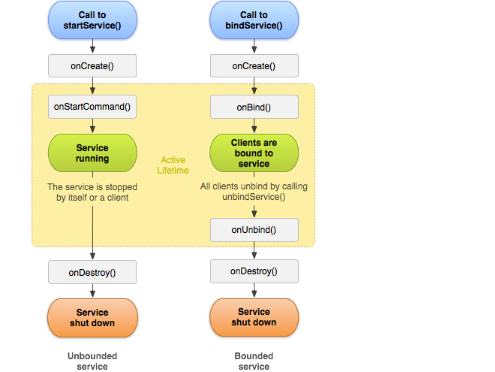
\includegraphics[width=.9\linewidth]{./pic/servicelifecycle.png}
\begin{itemize}
\item Service生命周期方法:
\begin{minted}[linenos=true]{java}
public class ExampleService extends Service {
    int mStartMode;       // 标识服务被杀死后的处理方式
    IBinder mBinder;      // 用于客户端绑定的接口
    boolean mAllowRebind; // 标识是否使用onRebind
    @Override
    public void onCreate() {
        // 服务正被创建
    }
    @Override
    public int onStartCommand(Intent intent, int flags, int startId) {
        // 服务正在启动,由startService()调用引发
        return mStartMode;
    }
    @Override
    public IBinder onBind(Intent intent) {
        // 客户端用bindService()绑定服务
        return mBinder;
    }
    @Override
    public boolean onUnbind(Intent intent) {
        // 所有的客户端都用unbindService()解除了绑定
        return mAllowRebind;
    }
    @Override
    public void onRebind(Intent intent) {
        // 某客户端正用bindService()绑定到服务,
        // 而onUnbind()已经被调用过了
    }
    @Override
    public void onDestroy() {
        // 服务用不上了,将被销毁
    }
}
\end{minted}
\begin{itemize}
\item 请注意onStartCommand()方法必须返回一个整数。这个整数是描述系统在杀死服务之后应该如何继续运行。onStartCommand()的返回值必须是以下常量之一:
\begin{itemize}
\item START\_NOT\_STICKY  
\begin{itemize}
\item 如果系统在onStartCommand()返回后杀死了服务,则不会重建服务了,除非还存在未发送的intent。 当服务不再是必需的,并且应用程序能够简单地重启那些未完成的工作时,这是避免服务运行的最安全的选项。 
\end{itemize}
\item START\_STICKY 
\begin{itemize}
\item 如果系统在onStartCommand()返回后杀死了服务,则将重建服务并调用onStartCommand(),但不会再次送入上一个intent, 而是用null intent来调用onStartCommand() 。除非还有启动服务的intent未发送完,那么这些剩下的intent会继续发送。 这适用于媒体播放器(或类似服务),它们不执行命令,但需要一直运行并随时待命。 
\end{itemize}
\item START\_REDELIVER\_INTENT 
\begin{itemize}
\item 如果系统在onStartCommand()返回后杀死了服务,则将重建服务并用上一个已送过的intent调用onStartCommand()。任何未发送完的intent也都会依次送入。这适用于那些需要立即恢复工作的活跃服务,比如下载文件。
\end{itemize}
\end{itemize}
\end{itemize}
\item 服务的生命周期与activity的非常类似。不过,更重要的是你需密切关注服务的创建和销毁环节,因为后台运行的服务是不会引起用户注意的。
\item 服务的生命周期——从创建到销毁——可以有两种路径:
\begin{itemize}
\item 一个started服务
\begin{itemize}
\item 这类服务由其它组件调用startService()来创建。然后保持运行,且必须通过调用stopSelf()自行终止。其它组件也可通过调用stopService() 终止这类服务。服务终止后,系统会把它销毁。
\item 如果一个Service被startService 方法多次启动,那么onCreate方法只会调用一次,onStart将会被调用多次(对应调用startService的次数),并且系统只会创建Service的一个实例(因此你应该知道只需要一次stopService调用)。该Service将会一直在后台运行,而不管对应程序的Activity是否在运行,直到被调用stopService,或自身的stopSelf方法。当然如果系统资源不足,android系统也可能结束服务。
\end{itemize}
\item 一个bound服务
\begin{itemize}
\item 服务由其它组件(客户端)调用bindService()来创建。然后客户端通过一个IBinder接口与服务进行通信。客户端可以通过调用unbindService()来关闭联接。多个客户端可以绑定到同一个服务上,当所有的客户端都解除绑定后,系统会销毁服务。(服务不需要自行终止。)
\item 如果一个Service被某个Activity 调用 Context.bindService 方法绑定启动,不管调用 bindService 调用几次,onCreate方法都只会调用一次,同时onStart方法始终不会被调用。当连接建立之后,Service将会一直运行,除非调用Context.unbindService 断开连接或者之前调用bindService 的 Context 不存在了(如Activity被finish的时候),系统将会自动停止Service,对应onDestroy将被调用。
\end{itemize}
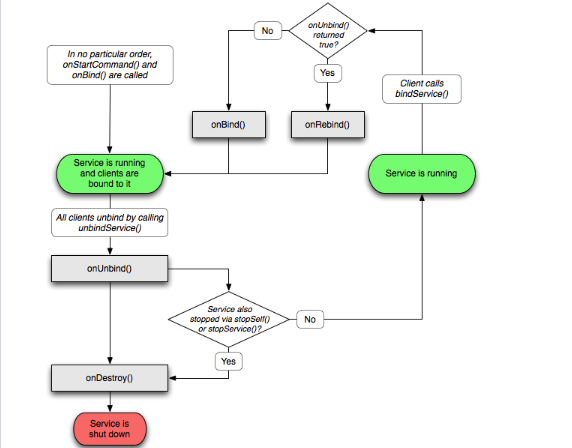
\includegraphics[width=.9\linewidth]{./pic/service2.png}
\end{itemize}
\item 这两条路径并不是完全隔离的。也就是说,你可以绑定到一个已经用startService()启动的服务上。例如,一个后台音乐服务可以通过调用startService()来启动,传入一个指明所需播放音乐的 Intent。 之后,用户也许需要用播放器进行一些控制,或者需要查看当前歌曲的信息,这时一个activity可以通过调用bindService()与此服务绑定。在类似这种情况下,stopService()或stopSelf()不会真的终止服务,除非所有的客户端都解除了绑定。
\begin{itemize}
\item 当在旋转手机屏幕的时候,当手机屏幕在“横”“竖”变换时,此时如果你的 Activity 如果会自动旋转的话,旋转其实是 Activity 的重新创建,因此旋转之前的使用 bindService 建立的连接便会断开(Context 不存在了)。
\end{itemize}
\end{itemize}
\subsection{在manifest中声明服务}
\label{sec-3-5}
\begin{itemize}
\item 无论是什么类型的服务都必须在manifest中申明,格式如下:
\begin{minted}[linenos=true]{xml}
<manifest ... >
  <application ... >
      <service android:name=".ExampleService" />
  </application>
</manifest>
\end{minted}
\item Service 元素的属性有:
\end{itemize}
\begin{center}
\begin{tabular}{ll}
\hline
android:name & 服务类名\\
android:label & 服务的名字.如果此项不设置,那么默认显示的服务名则为类名\\
android:icon & 服务的图标\\
android:permission & 申明此服务的权限,这意味着只有提供了该权限的应用才能控制或连接此服务\\
android:process & 表示该服务是否运行在另外一个进程,\\
 & 如果设置了此项,那么将会在包名后面加上这段字符串表示另一进程的名字\\
android:enabled & 如果此项设置为 true,那么 Service 将会默认被系统启动,不设置默认此项为 false\\
android:exported & 表示该服务是否能够被其他应用程序所控制或连接,不设置默认此项为 false \\
\hline
\end{tabular}
\end{center}
\begin{itemize}
\item android:name是唯一必需的属性——它定义了服务的类名。与activity一样,服务可以定义intent过滤器,使得其它组件能用隐式intent来调用服务。如果你想让服务只能内部使用(其它应用程序无法调用),那么就不必(也不应该)提供任何intent过滤器。
\item 此外,如果包含了android:exported属性并且设置为"false", 就可以确保该服务是你应用程序的私有服务。即使服务提供了intent过滤器,本属性依然生效。 
\end{itemize}
\subsection{startService 启动服务}
\label{sec-3-6}
\begin{itemize}
\item 从activity或其它应用程序组件中可以启动一个服务,调用startService()并传入一个Intent(指定所需启动的服务)即可。
\begin{minted}[linenos=true]{java}
  Intent intent = new Intent(this, MyService.class);
  startService(intent);
\end{minted}
\item 服务类:
\begin{minted}[linenos=true]{java}
public class MyService extends Service {
     // onBind 是 Service 的虚方法,因此我们不得不实现它。
     // 返回 null,表示客服端不能建立到此服务的连接。
    @Override
    public IBinder onBind(Intent intent) {
        // TODO Auto-generated method stub
        return null;
    }
    @Override
    public void onCreate() {
        super.onCreate();
    }
    @Override
    public int onStartCommand(Intent intent, int flags, int startId) {
        //接受传递过来的intent的数据 
        return START_STICKY; 
    };
    @Override
    public void onDestroy() {
        super.onDestroy();
    }
}
\end{minted}
\item 一个started服务必须自行管理生命周期。也就是说,系统不会终止或销毁这类服务,除非必须恢复系统内存并且服务返回后一直维持运行。 因此,服务必须通过调用stopSelf()自行终止,或者其它组件可通过调用stopService()来终止它。
\end{itemize}
\subsection{bindService 启动服务  }
\label{sec-3-7}
\begin{itemize}
\item 当应用程序中的activity或其它组件需要与服务进行交互,或者应用程序的某些功能需要暴露给其它应用程序时,你应该创建一个bound服务,并通过进程间通信(IPC)来完成。
\item 方法如下:
\begin{minted}[linenos=true]{java}
 Intent intent=new Intent(this,BindService.class); 
 bindService(intent, ServiceConnection conn, int flags)
\end{minted}
\item 注意bindService是Context中的方法,当没有Context时传入即可。
\item 在进行服务绑定的时,其flags有:
\begin{itemize}
\item Context.BIND\_AUTO\_CREATE    
\begin{itemize}
\item 表示收到绑定请求的时候,如果服务尚未创建,则即刻创建,在系统内存不足需要先摧毁优先级组件来释放内存,且只有驻留该服务的进程成为被摧毁对象时,服务才被摧毁 
\end{itemize}
\item Context.BIND\_DEBUG\_UNBIND     
\begin{itemize}
\item 通常用于调试场景中判断绑定的服务是否正确,但容易引起内存泄漏,因此非调试目的的时候不建议使用
\end{itemize}
\item Context.BIND\_NOT\_FOREGROUND     
\begin{itemize}
\item 表示系统将阻止驻留该服务的进程具有前台优先级,仅在后台运行。
\end{itemize}
\end{itemize}
\item 服务类:
\begin{minted}[linenos=true]{java}
public class BindService extends Service {
    // 实例化MyBinder得到mybinder对象;
    private final MyBinder binder = new MyBinder();
    // 返回Binder对象。
    @Override
    public IBinder onBind(Intent intent) {
        // TODO Auto-generated method stub
        return binder;
    }
     // 新建内部类MyBinder,继承自Binder(Binder实现IBinder接口),
     // MyBinder提供方法返回BindService实例。
    public class MyBinder extends Binder{
        public BindService getService(){
            return BindService.this;
        }
    }
    @Override
    public boolean onUnbind(Intent intent) {
        // TODO Auto-generated method stub
        return super.onUnbind(intent);
    }
}
\end{minted}
\item 启动服务的activity代码:
\begin{minted}[linenos=true]{java}
public class MainActivity extends Activity {
    // 是否绑定 
    boolean mIsBound = false; 
    BindService mBoundService;
    @Override
    protected void onCreate(Bundle savedInstanceState) {
        super.onCreate(savedInstanceState);
        setContentView(R.layout.activity_main);
        doBindService();
    }
    // 实例化ServiceConnection接口的实现类,用于监听服务的状态
    private ServiceConnection conn = new ServiceConnection() {  
            @Override  
            public void onServiceConnected(ComponentName name, IBinder service) {  
                BindService mBoundService = ((BindService.MyBinder) service).getService();  
            
            }  
            @Override  
            public void onServiceDisconnected(ComponentName name) {  
                mBoundService = null;  
            }  
        }; 
    // 绑定服务 
    public void doBindService() {  
        bindService(new Intent(MainActivity.this, BindService.class), conn,Context.BIND_AUTO_CREATE);  
        mIsBound = true;  
    }  
    // 解除绑定服务
    public void doUnbindService() {  
        if (mIsBound) {  
            // Detach our existing connection.  
            unbindService(conn);  
            mIsBound = false;  
        }  
    } 
    @Override
    protected void onDestroy() {
        // TODO Auto-generated method stub
        super.onDestroy();
        doUnbindService();
    }
}
\end{minted}
\item 注意在AndroidMainfest.xml中对Service进行显式声明
\item 判断Service是否正在运行:
\begin{minted}[linenos=true]{java}
private boolean isServiceRunning() {
    ActivityManager manager = (ActivityManager) getSystemService(ACTIVITY_SERVICE);
    {
        if ("com.example.demo.BindService".equals(service.service.getClassName())) {
            return true;
        }
    }
    return false;
}
\end{minted}
\end{itemize}
\section{IntentService使用详解和实例但介绍}
\label{sec-4}
\subsection{IntentService定义}
\label{sec-4-1}
\begin{itemize}
\item IntentService继承与Service,用来处理异步请求。客户端可以通过startService(Intent)方法传递请求给IntentService。IntentService在onCreate()函数中通过HandlerThread单独开启一个线程来依次处理所有Intent请求对象所对应的任务。 
\item 这样以免事务处理阻塞主线程(ANR)。执行完所一个Intent请求对象所对应的工作之后,如果没有新的Intent请求达到,则 \textbf{自动停止} Service;否则执行下一个Intent请求所对应的任务。 
\item IntentService在处理事务时,还是采用的Handler方式,创建一个名叫ServiceHandler的内部Handler,并把它直接绑定到HandlerThread所对应的子线程。 ServiceHandler把处理一个intent所对应的事务都封装到叫做 \textbf{onHandleIntent} 的虚函数;因此我们直接实现虚函数onHandleIntent,再在里面根据Intent的不同进行不同的事务处理就可以了。
\item 另外,IntentService默认实现了Onbind()方法,返回值为null。
\item 使用IntentService需要实现的两个方法:
\begin{itemize}
\item 构造函数 
\begin{itemize}
\item IntentService的构造函数一定是 \textbf{参数为空} 的构造函数,然后再在其中调用super("name")这种形式的构造函数。因为Service的实例化是系统来完成的,而且系统是用参数为空的构造函数来实例化Service的
\end{itemize}
\item 实现虚函数onHandleIntent
\begin{itemize}
\item 在里面根据Intent的不同进行不同的事务处理。 
\item 好处:处理异步请求的时候可以减少写代码的工作量,比较轻松地实现项目的需求。
\end{itemize}
\end{itemize}
\end{itemize}
\subsection{IntentService与Service的区别}
\label{sec-4-2}
\begin{itemize}
\item Service不是独立的进程,也不是独立的线程,它是依赖于应用程序的主线程的,不建议在Service中编写耗时的逻辑和操作,否则会引起ANR。
\item IntentService 它创建了一个独立的工作线程来处理所有的通过onStartCommand()传递给服务的intents(把intent插入到工作队列中)。通过工作队列把intent逐个发送给onHandleIntent()。 
\item 不需要主动调用stopSelft()来结束服务。因为,在所有的intent被处理完后,系统会自动关闭服务。
\item 默认实现的onBind()返回null。
\end{itemize}
\subsection{IntentService实例介绍}
\label{sec-4-3}
\begin{itemize}
\item 首先是myIntentService.java
\begin{minted}[linenos=true]{java}
public class myIntentService extends IntentService {
    //------------------必须实现-----------------------------
    public myIntentService() {
        super("myIntentService");
        // 注意构造函数参数为空,这个字符串就是worker thread的名字
    }
    @Override
    protected void onHandleIntent(Intent intent) {
        //根据Intent的不同进行不同的事务处理 
        String taskName = intent.getExtras().getString("taskName");  
        switch (taskName) {
        case "task1":
            Log.i("myIntentService", "do task1");
            break;
        case "task2":
            Log.i("myIntentService", "do task2");
            break;
        default:
            break;
        }        
    }
    //--------------------用于打印生命周期--------------------    
    @Override
    public void onCreate() {
        Log.i("myIntentService", "onCreate");
        super.onCreate();
    }
    @Override
    public int onStartCommand(Intent intent, int flags, int startId) {
        Log.i("myIntentService", "onStartCommand");
        return super.onStartCommand(intent, flags, startId);
    }
    @Override
    public void onDestroy() {
        Log.i("myIntentService", "onDestroy");
        super.onDestroy();
    }
}
\end{minted}
\item 然后记得在Manifest.xml中注册服务
\begin{minted}[linenos=true]{xml}
<service android:name=".myIntentService">
  <intent-filter >  
    <action android:name="cn.scu.finch"/>  
  </intent-filter>     
</service>
\end{minted}
\item 最后在Activity中开启服务
\begin{minted}[linenos=true]{java}
public class MainActivity extends Activity {
    @Override
    protected void onCreate(Bundle savedInstanceState) {
        // TODO Auto-generated method stub
        super.onCreate(savedInstanceState);
        //同一服务只会开启一个worker thread,在onHandleIntent函数里依次处理intent请求。
        Intent i = new Intent("cn.scu.finch");  
        Bundle bundle = new Bundle();  
        bundle.putString("taskName", "task1");  
        i.putExtras(bundle);  
        startService(i);  
        Intent i2 = new Intent("cn.scu.finch");  
        Bundle bundle2 = new Bundle();  
        bundle2.putString("taskName", "task2");  
        i2.putExtras(bundle2);  
        startService(i2); 
        startService(i);  //多次启动
    }
}
\end{minted}
\item 运行结果:
\begin{minted}[linenos=true]{text}
myIntentService onCreate()
myIntentService onStartCommand()
myIntentService onStartCommand()
myIntentService do task1
myIntentService onStartCommand()
myIntentService do task2
myIntentService do task1
myIntentService onDestroy()
\end{minted}
\item IntentService在onCreate()函数中通过HandlerThread单独开启一个线程来依次处理所有Intent请求对象所对应的任务。 
\item 通过onStartCommand()传递给服务intent被**依次**插入到工作队列中。工作队列又把intent逐个发送给onHandleIntent()。
\item 注意:
\begin{itemize}
\item 它只有一个工作线程,名字就是构造函数的那个字符串,也就是“myIntentService”,我们知道多次开启service,只会调用一次onCreate方法(创建一个工作线程),多次onStartCommand方法(用于传入intent通过工作队列再发给onHandleIntent函数做处理)。
\end{itemize}
\end{itemize}

\section{Android启动过程图解}
\label{sec-5}
\begin{itemize}
\item Android手机开机执行过程图:
\end{itemize}

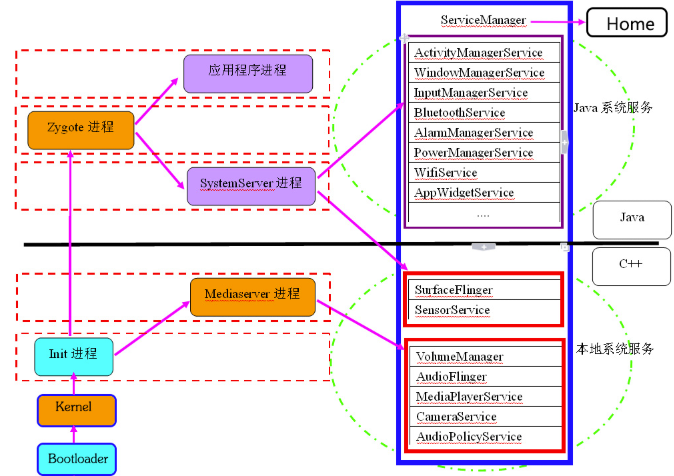
\includegraphics[width=.9\linewidth]{./pic/androidStart.png}
\begin{itemize}
\item 从开机到桌面的过程为:
\begin{itemize}
\item Bootloader ---> Kernel ---> Init进程 ---> Zygote ---> SystemServer ---> ServiceManager ---> Home Launcher
\end{itemize}
\item Android服务包括系统服务和应用服务,系统服务是指Android系统在启动过程就已经启动实现了的服务,对于系统服务又分为Java服务和本地服务,Java服务是由Java代码编写而成,由SystemServer进程提供,而本地服务是由C/C++实现的服务,由Init进程在系统启动时启动的服务。应用服务是由开发者自行实现的某些特定服务。
\end{itemize}
\subsubsection{Bootloader}
\label{sec-5-0-1}
\begin{itemize}
\item 当电源按下,引导芯片代码开始从预定义的地方(固化在ROM)开始执行。加载引导程序到RAM,然后执行。
\item BootLoader是在操作系统内核运行之前运行。可以初始化硬件设备、建立内存空间映射图,从而将系统的软硬件环境带到一个合适状态,以便为最终调用操作系统内核准备好正确的环境。
\end{itemize}
\subsubsection{Kernel}
\label{sec-5-0-2}
\begin{itemize}
\item Android内核启动时,会设置缓存、被保护存储器、计划列表,加载驱动。当内核完成系统设置,它首先在系统文件中寻找”init”文件,然后启动root进程或者系统的第一个进程。
\end{itemize}
\subsubsection{init进程}
\label{sec-5-0-3}
\begin{itemize}
\item init进程,它是一个由内核启动的用户级进程。内核自行启动(已经被载入内存,开始运行,并已初始化所有的设备驱动程序和数据结构等)之后,就通过启动一个用户级程序init的方式,完成引导进程。init始终是第一个进程。
\item 启动过程就是代码init.c中main函数执行过程:system\core\init\init.c在函数中执行了: \textbf{文件夹建立} , \textbf{挂载} , \textbf{rc文件解析} , \textbf{属性设置} , \textbf{启动服务} , \textbf{执行动作} , \textbf{socket监听} 
\begin{itemize}
\item rc文件解析
\begin{itemize}
\item .rc文件是Android使用的初始化脚本文件 ,Android中有特定的格式以及规则。
\end{itemize}
\end{itemize}
\end{itemize}
\subsubsection{Zygote}
\label{sec-5-0-4}
\begin{itemize}
\item 所有的应用程序进程以及系统服务进程(SystemServer)都是由Zygote进程孕育(fork)出来的,zygote本身是Native应用程序,与驱动内核无关。
\item 我们知道,Android系统是基于Linux内核的,而在Linux系统中,所有的进程都是init进程的子孙进程,也就是说,所有的进程都是直接或者间接地由init进程fork出来的。Zygote进程也不例外,它是在系统启动的过程,由init进程创建的(在系统启动脚本system/core/rootdir/init.rc文件中)。
\item 在Java中,不同的虚拟机实例会为不同的应用分配不同的内存。假如Android应用应该尽可能快地启动,但如果Android系统为每一个应用启动不同的Dalvik虚拟机实例,就会消耗大量的内存以及时间。因此,为了克服这个问题,Android系统创造了”Zygote”。Zygote是一个虚拟器进程,预加载以及初始化核心库类,让Dalvik虚拟机共享代码、降低内存占用和启动时间。
\end{itemize}
\begin{enumerate}
\item Zygote进程包含两个主要模块
\label{sec-5-0-4-1}
\begin{itemize}
\item ①Socket服务端,该Socket服务端用于接收启动新的Dalvik进程命令。
\item ②Framework共享类及共享资源,当Zygote进程启动后,会装载一些共享类和资源,共享类是在preload-classes文件中定义的,共享资源是在preload-resources文件中定义。因为其他Dalvik进程是由Zygote进程孵化出来的,因此只要Zygote装载好了这些类和资源后,新的Dalvik进程就不需要在装载这些类和资源了,它们共享Zygote进程的资源和类。
\end{itemize}
\item Zygote启动分为两个阶段
\label{sec-5-0-4-2}
\begin{itemize}
\item ① \textbf{虚拟机启动 --- 通过native启动}
\begin{itemize}
\item startVm(\&mJavaVM, \&env)   启动虚拟机 
\item onVmCreated(env)         虚拟机启动后的初始化
\item startReg(env)             注册JNI函数
\item env->CallStaticVoidMethod(startClass, startMeth, strArray) 调用ZygoteInit类的main函数开创java世界 
\end{itemize}
\item ② \textbf{SystemServer进程 --- 通过Java启动}
\begin{itemize}
\item registerZygoteSocket()  为zygote进程注册监听socket
\item preload()            加载常用的JAVA类和系统资源
\item startSystemServer()    启动SystemServer进程
\item runSelectLoopMode()  进入循环监听模式
\item closeServerSocket()    进程退出时,关闭socket监听
\end{itemize}
\end{itemize}
\end{enumerate}
\subsubsection{启动系统服务}
\label{sec-5-0-5}
\begin{itemize}
\item Zygote创建新的进程去启动系统服务。你可以在ZygoteInit类的”startSystemServer”方法中找到源代码。
\item 核心服务:
\begin{itemize}
\item 启动电源管理器; 
\end{itemize}
\item 创建Activity管理器; 
\begin{itemize}
\item 启动电话注册; 
\item 启动包管理器;
\item 设置Activity管理服务为系统进程;
\item 启动上下文管理器;
\item 启动系统Context Providers;
\item 启动电池服务;
\item 启动定时管理器;
\item 启动传感服务;
\item 启动窗口管理器;
\item 启动蓝牙服务;
\item 启动挂载服务。
\end{itemize}
\item 其他服务:
\end{itemize}
\subsubsection{引导完成}
\label{sec-5-0-6}
\begin{itemize}
\item 一旦系统服务在内存中跑起来了,Android就完成了引导过程。在这个时候“ACTION\_BOOT\_COMPLETED”开机启动广播就会发出去。
\end{itemize}

\section{AIDL的使用情况和实例介绍}
\label{sec-6}
\subsection{AIDL是什么?}
\label{sec-6-1}
\begin{itemize}
\item AIDL (Android Interface Definition Language), Android接口定义语言,Android提供的IPC (Inter Process Communication,进程间通信)的一种独特实现。
\end{itemize}
\subsection{什么情况下要使用AIDL}
\label{sec-6-2}
\begin{itemize}
\item 使用AIDL只有在你允许来自不同应用的客户端跨进程通信访问你的service,并且想要在你的service种处理**多线程**的时候才是必要的。 如果你不需要执行不同应用之间的IPC并发,你应该通过实现Binder建立你的接口,或者如果你想执行IPC,但是不需要处理多线程。那么使用Messenger实现你的接口。
\end{itemize}
\subsection{定义一个AIDL接口的步骤}
\label{sec-6-3}
\begin{itemize}
\item 必须在一个.aidl文件中使用java编程语言语法定义你的AIDL接口,然后在提供service的应用中和任何绑定到这个service的应用中的源代码中(在src目录吓)保存它。
\item 当你编译包含.aidl文件的应用时,Android SDK工具基于这个.aidl文件生成一个IBinder接口,并且把它保存到项目的gen目录吓.service必须恰当的实现这个IBinder接口 之后客户端应用可以绑定到这个服务上,然后从IBinder调用方法来执行IPC。
\item 使用AIDL建立一个邻接的service需要遵循下面的步骤:
\begin{itemize}
\item 1. 建立.aidl文件 
\begin{itemize}
\item 这个文件使用方法签名定义了语言接口 
\end{itemize}
\item 2.实现这个接口 
\begin{itemize}
\item Android SDk工具基于你的.aidl文件使用java语言生成一个接口 这个接口有一个内部抽象类,叫做Stub,它是继承Binder并且实现你AIDL接口的 你必须继承这个Stub类并且实现这些方法
\end{itemize}
\item 3.暴露这个接口给客户端 
\begin{itemize}
\item 实现一个service并且覆盖onBind()方法返回你的Stub实现类。
\end{itemize}
\item 你的.aidl文件必须被复制到其他应用程序中来让他们访问你service的接口,你必须维护原始接口的支持(向后兼容)。
\end{itemize}
\end{itemize}
\subsection{用一个实例来分步骤说明}
\label{sec-6-4}
\subsubsection{在server项目中建立.aidl文件 }
\label{sec-6-4-1}
![这里写图片描述](\url{http://img.blog.csdn.net/20160504180944041})
\begin{itemize}
\item AIDL使用一个简单的语法让你声明一个带有一个或者多个带有参数和返回值方法的接口 参数和返回值可以是任何类型,甚至是AIDL生成的接口。
\item IService.aidl
\begin{minted}[linenos=true]{java}
package com.example.aidl;
interface IService {
    String hello(String name); 
}
\end{minted}
\end{itemize}
\subsubsection{在server项目中建立服务类}
\label{sec-6-4-2}
\begin{itemize}
\item 当你编译你的应用时,Android SDK工具生成一个.java接口文件用你的.aidl文件命名生成的接口包含一个名字为Stub的子类,这是一个它父类的抽象实现,并且声明了.aidl中所有的方法。
\item Stub也定义了一些辅助的方法,最显著的就是asInterface(),它是用来接收一个IBinder(通常IBinder传递给客户端的onServiceConnected()回调方法)并且返回一个Stub接口的实例 。
\item 一旦你为service实现了接口,你需要把它暴露给客户端,这样他们才能绑定到上面 为了给你的service暴露接口,继承Service并且实现onBind()方法返回一个你实现生成的Stub类。
\item AIDLService.java
\begin{minted}[linenos=true]{java}
public class AIDLService extends Service {
    @Override
    public void onCreate() {
        super.onCreate();
    }
    @Override
    public IBinder onBind(Intent intent) {
        // Return the interface
        return new IService.Stub() {
            @Override
            public String hello(String name) throws RemoteException {
                // TODO Auto-generated method stub
                return "hello"+name;
            }
        };
    }
}
\end{minted}
\end{itemize}
\subsubsection{在server项目AndroidManifest中申明Service}
\label{sec-6-4-3}
\begin{minted}[linenos=true]{xml}
<service 
    android:name="com.example.service.AIDLService" >
  <intent-filter>  
    <action android:name="android.intent.action.AIDLService" />  
  </intent-filter> 
</service>
\end{minted}
\subsubsection{把server项目中的aidl文件带包拷贝到client项目中(包名要相同)}
\label{sec-6-4-4}
![这里写图片描述](\url{http://img.blog.csdn.net/20160504181850678}) 
\begin{itemize}
\item MainActivity.java
\begin{minted}[linenos=true]{java}
public class MainActivity extends Activity {
    IService RemoteService; //监听服务
    private ServiceConnection mConnection = new ServiceConnection() {
            @Override
            public void onServiceConnected(ComponentName name, IBinder service) {
                // TODO Auto-generated method stub
                Log.i("mConnection", service+"");
                RemoteService = IService.Stub.asInterface(service);
            
                try {
                    String s= RemoteService.hello("finch");
                    Toast.makeText(MainActivity.this, s, Toast.LENGTH_LONG).show();
                } catch (RemoteException e) {
                    e.printStackTrace();
                }
            }
            @Override
            public void onServiceDisconnected(ComponentName name) {
                // TODO Auto-generated method stub
            }
        };
    @Override
    protected void onCreate(Bundle savedInstanceState) {
        super.onCreate(savedInstanceState);
        setContentView(R.layout.activity_main);
        
        initService();
    }
    // 连接服务
    private void initService() {
        Intent i = new Intent( );
        i.setAction("android.intent.action.AIDLService");
        boolean ret = bindService(i, mConnection, Context.BIND_AUTO_CREATE);
    }
    // 断开服务
    private void releaseService() {
        unbindService(mConnection);
        mConnection = null;
    }
    @Override
    protected void onDestroy() {
        super.onDestroy();
        releaseService();
    }
}
\end{minted}
\item 运行结果:
\begin{minted}[linenos=true]{java}
<img src="http://img.blog.csdn.net/20160504182305682" width="286" height="473" />
\end{minted}
\end{itemize}
[文章中AIDL例子代码下载](\url{http://download.csdn.net/detail/amazing7/9510133})
% Emacs 26.1 (Org mode 8.2.7c)
\end{document}